\part{Graph and Network Theory}
	\chapter{Paths, Trees, and Cycles}

	\chapter{Shortest-Path Problem}

	\chapter{Minimum Spanning Tree Problem}

	\chapter{Maximum Flow Problem}

	\chapter{Minimum Cost Flow Problem}

	\chapter{Assignment and Matching Problem}

	\chapter{Graph Algorithms}

	\chapter{Polygon Triangulation}
		\section{Types of Polygons}
			\framebox{\textbf{Def:}} A \textbf{simple polygon} is a closed polygonal curve without self-intersection.\\
			\begin{figure}[h!]
				\centering
				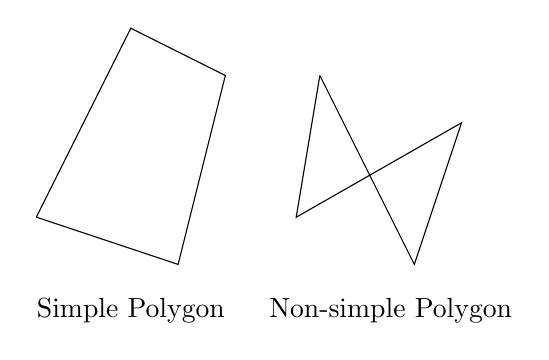
\begin{tikzpicture}[scale=0.6]
					\draw (0, 0) -- (3, -1) -- (4, 3) -- (2, 4) -- (0, 0);
					\draw (6, 3) -- (8, -1) -- (9, 2) -- (5.5, 0) -- (6, 3);
					\node at (2, -1.5) [below] {Simple Polygon};
					\node at (7.5, -1.5) [below] {Non-simple Polygon};
				\end{tikzpicture}
			\end{figure}\\
			Polygons are basic building blocks in most geometric applications. It can model arbitrarily complex shapes, and apply simple algorithms and algebraic representation/manipulation.
			
		\section{Triangulation}
			\framebox{\textbf{Def:}} \textbf{Triangulation} is to partition polygon $P$ into non-overlapping triangles using diagonals only. It reduces complex shapes to collection of simpler shapes. Every simple $n$-gon admits a triangulation which has $n-2$ triangles.\\
			\begin{figure}[h!]
				\centering
				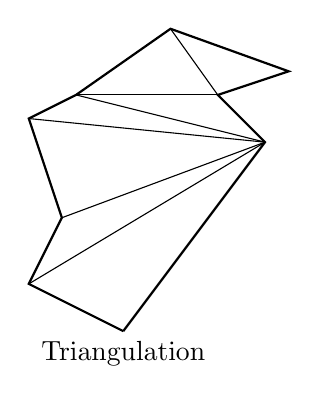
\begin{tikzpicture}[scale=0.6]
					\draw [thick] (0, 0) -- (3, 4) -- (2, 5) -- (3.5, 5.5) -- (1, 6.4) -- (-1, 5) -- (-2, 4.5) -- (-1.3, 2.4) -- (-2, 1) -- (0, 0);
					\draw (-2, 1) -- (3, 4);
					\draw (-1.3, 2.4) -- (3, 4);
					\draw (-2, 4.5) -- (3, 4);
					\draw (-1, 5) -- (3, 4);
					\draw (-1, 5) -- (2, 5);
					\draw (2, 5) -- (1, 6.4);
					\node at (0, 0) [below] {Triangulation};
				\end{tikzpicture}
			\end{figure}\\
			\framebox{\textbf{Theorem:}} Every polygon has a triangulation\\  
			\framebox{\textbf{Lemma:}} Every polygon with more than three vertices has a diagonal.\\
			\framebox{\textbf{Proof:}}(by Meisters, 1975) Let $P$ be a polygon with more than three vertices. Every vertex of a $P$ is either \textit{convex} or \textit{concave}. W.L.O.G.(any polygon must has convex corner) Assume $p$ is a convex vertex. Denote the neighbors of $p$ as $q$ and $r$. If $\bar{qr}$ is a diagonal, done, and we call $\triangle{pqr}$ is an \textit{ear}. If $\triangle{pqr}$ is not an ear, it means at least one vertex is inside $\triangle{pqr}$, assume among those vertexes inside $\triangle{pqr}$, $s$ is a vertex closest to $p$, then $\bar{ps}$ is a diagonal. 
			
		\section{Art Gallery Theorem}
			\framebox{\textbf{Problem:}} The floor plan of an art gallery modeled as a simple polygon with $n$ vertices, there are guards which is stationed at fixed positions with 360 degree vision but cannot see through the walls. How many guards does the art gallery need for the security? (Fun fact: This problem was posted to Vasek Chvatal by Victor Klee in 1973)\\
			\framebox{\textbf{Theorem:}} Every $n$-gon can be guarded with $\lfloor \frac{n}{3} \rfloor$ vertex guards\\
			\framebox{\textbf{Lemma:}} Triangulation graph can be 3-colored.\\
			\framebox{\textbf{Proof:}} \\
			- $P$ plus triangulation is a planar graph\\
			- 3-coloring means there exist a 3-partition for vertices that no edge or diagonal has both endpoints within the same set of vertices.\\
			- Proof by Induction:\\
			\indent - Remove an ear (there will always exist ear) \\
			\indent - Inductively 3-color the rest\\
			\indent - Put ear back, coloring new vertex with the label not used by the boundary diagonal.

		\section{Triangulation Algorithms}

		\section{Shortest Path}


